% ======================================================================
% BLOQUE 5 — Neutrinos, IceCube y astronomía multimensajero
% ======================================================================
\section{Neutrinos e IceCube}
\bloque{NEUTRINOS}

% ---------------------------------------------------------------- 41
\begin{frame}[plain]
  \fondo[0.0]{halzen/halzen_p005_sintexto.jpg}
  \velo[0.9]{b}
  \begin{tikzpicture}[remember picture, overlay]
    \node[anchor=north west, text=white, font=\Large\bfseries]
      at ([xshift=0.6cm, yshift=-0.35cm]current page.north west)
      {¿Por qué neutrinos? La portada, explicada};
    \tikzset{rot/.style={font=\small\bfseries, align=left, text=white}}
    \node[rot, anchor=south] at ([xshift=8.7cm, yshift=7.2cm]current page.south west)
      {$p$: desviado por campos magnéticos};
    \node[rot, anchor=south west] at ([xshift=9.2cm, yshift=4.7cm]current page.south west)
      {$\gamma$: absorbido\\{\footnotesize $\gamma\gamma_\mathrm{fondo}\to e^+e^-$}};
    \node[rot, anchor=north, text=hielo] at ([xshift=9.0cm, yshift=3.6cm]current page.south west)
      {$\nu$: en línea recta y sin absorberse};
    \node[anchor=south west, text width=14.6cm, align=left, text=white, font=\small]
      at ([xshift=0.6cm, yshift=0.35cm]current page.south west) {%
      \textbf{Neutros}: no se desvían. \textbf{Interacción débil}: escapan de
      ambientes opacos a la luz. Se producen en \textbf{interacciones hadrónicas}:
      señalan dónde se aceleran protones y núcleos.\\[2pt]
      El precio: $\sigma_{\nu N}(1\,\mathrm{PeV})\sim10^{-33}\,\mathrm{cm^2}$,
      \;$\lambda$ en hielo $\sim2\times10^{4}$\,km: \textbf{en un km de hielo
      interactúa uno de cada $\sim$20.000.}};
  \end{tikzpicture}
  \creditoblanco{Composición: F.~Halzen, Erice 2024}
\end{frame}

% ---------------------------------------------------------------- 42
\begin{frame}{De dónde salen los neutrinos astrofísicos}
  \begin{columns}[c,onlytextwidth]
    \column{0.55\textwidth}
      \centering
      \begin{tikzpicture}[x=1cm,y=1cm]
        \node[font=\small\bfseries, text=itedaOrange] (p) at (0,1.5) {$p$};
        \node[font=\small, align=center] (t) at (0,0) {$p$ (gas)\\o $\gamma$ (luz)};
        \node[circle, fill=itedaLight, draw=itedaTeal, inner sep=2pt, font=\scriptsize] (v) at (1.6,0.75) {choque};
        \draw[flecha] (p) -- (v); \draw[flecha] (t) -- (v);
        \node[font=\small] (pi0) at (3.3,1.7) {$\pi^0$};
        \node[font=\small] (pic) at (3.3,-0.2) {$\pi^\pm$};
        \draw[flecha] (v) -- (pi0); \draw[flecha] (v) -- (pic);
        \node[font=\small, text=cmbAzul, anchor=west] (gg) at (4.4,1.7) {$\gamma\,\gamma$};
        \draw[flecha, cmbAzul] (pi0) -- (gg);
        \node[font=\small, anchor=west] (mu) at (4.4,0.4) {$\mu^\pm$};
        \node[font=\small, text=violetaNu, anchor=west] (n1) at (4.4,-0.8) {$\nu_\mu$};
        \draw[flecha] (pic) -- (mu.west); \draw[flecha, violetaNu] (pic) -- (n1.west);
        \node[font=\small, text=violetaNu, anchor=west] at (5.4,0.4) {$\to e^\pm\,\nu_e\,\nu_\mu$};
      \end{tikzpicture}\\[6pt]
      \small
      \[ E_\nu\approx\tfrac{1}{20}E_p, \qquad E_\gamma\approx\tfrac{1}{10}E_p \]
      {\footnotesize Sabores en la fuente $\nu_e:\nu_\mu:\nu_\tau\approx1:2:0$;
      tras oscilar en el viaje, $\approx1:1:1$ en la Tierra.}
    \column{0.42\textwidth}
      \begin{clave}
        \textbf{Por cada neutrino, un fotón gamma}: los mismos piones producen
        ambos. Si una fuente emite neutrinos sin los gammas esperados, la
        fuente es \textbf{opaca} a la luz.
      \end{clave}
      \vspace{4pt}
      {\footnotesize Un neutrino es la firma de \textbf{hadrones} acelerados;
      un gamma puede venir también de electrones (Compton inverso).}
  \end{columns}
\end{frame}

% ---------------------------------------------------------------- 43
\begin{frame}{Auger también busca neutrinos}
  \begin{columns}[c,onlytextwidth]
    \column{0.56\textwidth}
      \centering
      \begin{tikzpicture}[x=1cm,y=1cm]
        \fill[itedaGray!25] (-0.5,-1.2) -- (7,-1.2) -- (7,-0.2) -- (5.6,-0.2) --
          (4.6,0.9) -- (3.8,0.4) -- (3.0,-0.2) -- (-0.5,-0.2) -- cycle;
        \node[font=\tiny, text=itedaGray] at (4.4,0.2) {Andes};
        \draw[itedaTeal, thick] (-0.5,-0.2) -- (7,-0.2);
        \foreach \x in {0,0.6,...,2.4}{\fill[itedaTeal] (\x,-0.2) rectangle ++(0.18,0.12);}
        \draw[violetaNu, thick, dashed] (7.0,-0.75) -- (4.0,-0.55);
        \node[font=\scriptsize, text=violetaNu, anchor=south east] at (7.0,-0.75) {$\nu_\tau$};
        \draw[cmbRojo, thick, -{Stealth}] (4.0,-0.55) -- (3.2,-0.25)
          node[pos=0.3, below, font=\scriptsize] {$\tau$};
        \fill[itedaOrange] (3.1,-0.18) circle (1.5pt);
        \fill[itedaOrange!30] (3.1,-0.18) -- (0.2,0.35) -- (0.2,-0.18) -- cycle;
        \node[font=\scriptsize, align=center] at (2.1,0.75) {lluvia que «sube»\\casi horizontal};
        \draw[itedaTealDark, thick, -{Stealth}] (-0.4,2.5) -- (0.5,-0.1);
        \node[font=\scriptsize, align=left, anchor=west] at (-0.1,2.4)
          {$\nu$ descendente muy inclinado:\\lluvia \textbf{joven}, rica en $e^\pm$};
      \end{tikzpicture}\\[4pt]
      {\footnotesize Rozando la Tierra (y los Andes), un $\nu_\tau$ produce un
      $\tau$ que decae en el aire.}
    \column{0.41\textwidth}
      \small
      Las lluvias de rayos cósmicos muy inclinados llegan \textbf{viejas}:
      sólo muones. Una lluvia inclinada \textbf{joven} delata a un neutrino.
      \vspace{4pt}
      \begin{clave}
        Sin candidatos hasta hoy: límites entre los más restrictivos a EeV, y
        búsquedas en coincidencia con ondas gravitacionales (GW170817).
      \end{clave}
      {\footnotesize\color{itedaGray} Auger es un observatorio de
      lluvias, no un telescopio de neutrinos: su sensibilidad empieza en
      $\sim10^{17}$\,eV.}
  \end{columns}
  \creditoizq{Esquema ilustrativo, sin escala}
\end{frame}

% ---------------------------------------------------------------- 43b
\begin{frame}[plain]
  \fondo[0.0]{halzen/polo_sur_avion.jpg}
  \velo[0.7]{t}
  \begin{tikzpicture}[remember picture, overlay]
    \node[anchor=north west, text=white, align=left, text width=13cm]
      at ([xshift=0.6cm, yshift=-0.45cm]current page.north west) {%
      {\Large\bfseries El Polo Sur, desde un avión}\\[4pt]
      {\small Ese puntito es la base Amundsen--Scott, con el laboratorio de
      IceCube. Abajo hay casi \textbf{3\,km de hielo}, ultratransparente por
      debajo de 1,35\,km de profundidad.}};
    \draw[itedaOrange, very thick, -{Stealth[length=3mm]}]
      ([xshift=-4.2cm, yshift=-1.6cm]current page.center) -- ([xshift=-2.3cm, yshift=-0.35cm]current page.center);
    \node[text=white, font=\small\bfseries, anchor=north east, fill=black, fill opacity=0.45,
      text opacity=1, inner sep=2pt]
      at ([xshift=-4.1cm, yshift=-1.6cm]current page.center) {IceCube};
  \end{tikzpicture}
  \creditoblanco{Foto: vía F.~Halzen, Erice 2024}
\end{frame}

% ---------------------------------------------------------------- 44
\bloque{NEUTRINOS · ICECUBE}
\begin{frame}[plain]
  \fondo[0.1]{halzen/icecube_lab_aurora.jpg}
  \velo[0.85]{l}
  \begin{tikzpicture}[remember picture, overlay]
    \node[anchor=north west, text=white, align=left, text width=6.6cm]
      at ([xshift=0.6cm, yshift=-0.6cm]current page.north west) {%
      {\Large\bfseries IceCube: un kilómetro cúbico de hielo antártico}\\[10pt]
      \small\color{white}
      \begin{itemize}\small\color{white}
        \item 86 cuerdas, \textbf{5160 módulos ópticos} entre 1450 y 2450\,m de
          profundidad.
        \item Hielo ultratransparente: longitud de absorción de 100 a 250\,m.
        \item Completado en 2010; en el techo, IceTop mide lluvias.
      \end{itemize}};
    \node[anchor=east, fill=white, rounded corners=3pt, inner sep=3pt]
      at ([xshift=-0.5cm, yshift=-0.2cm]current page.east)
      {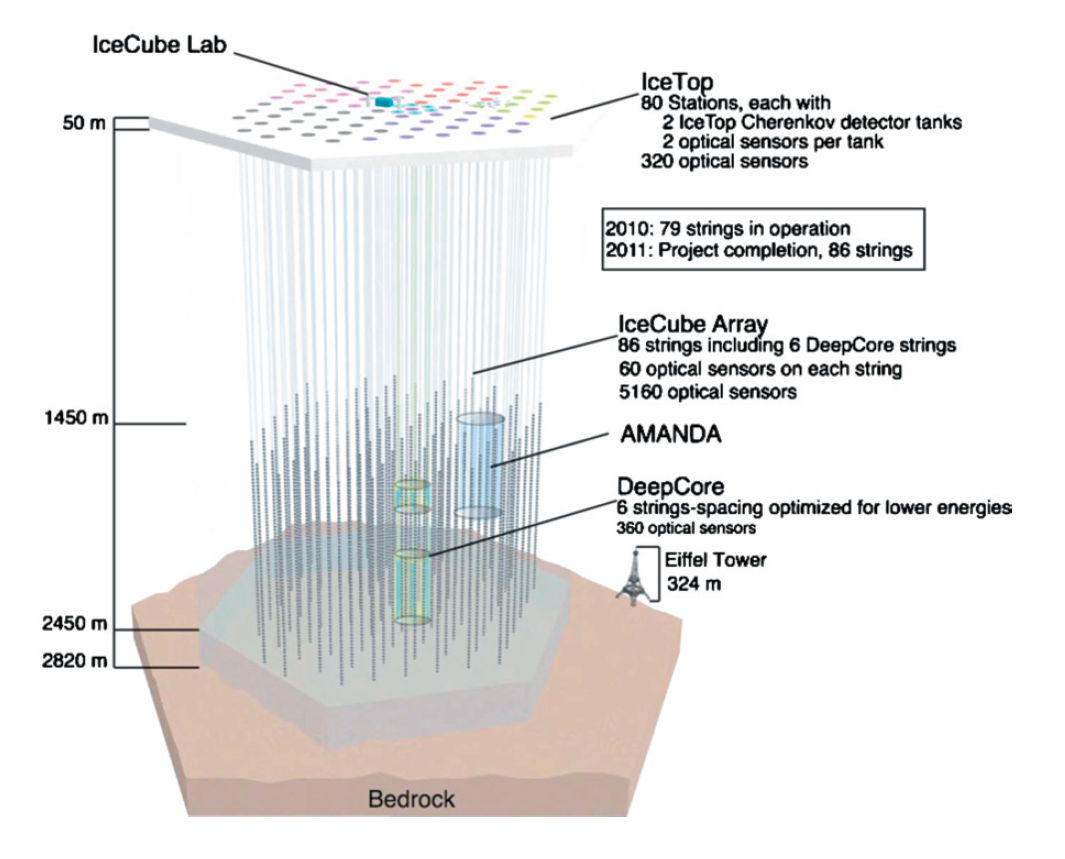
\includegraphics[height=6.1cm]{externas/icecube_arquitectura.png}};
  \end{tikzpicture}
  \creditoblanco{Foto: IceCube/NSF, vía F.~Halzen (2024). Diagrama: IceCube, CC BY 3.0 (Wikimedia Commons)}
\end{frame}

% ---------------------------------------------------------------- 45
\begin{frame}{Premio Nobel de Física 2026: Francis Halzen}
  \begin{columns}[c,onlytextwidth]
    \column{0.55\textwidth}
      \centering
      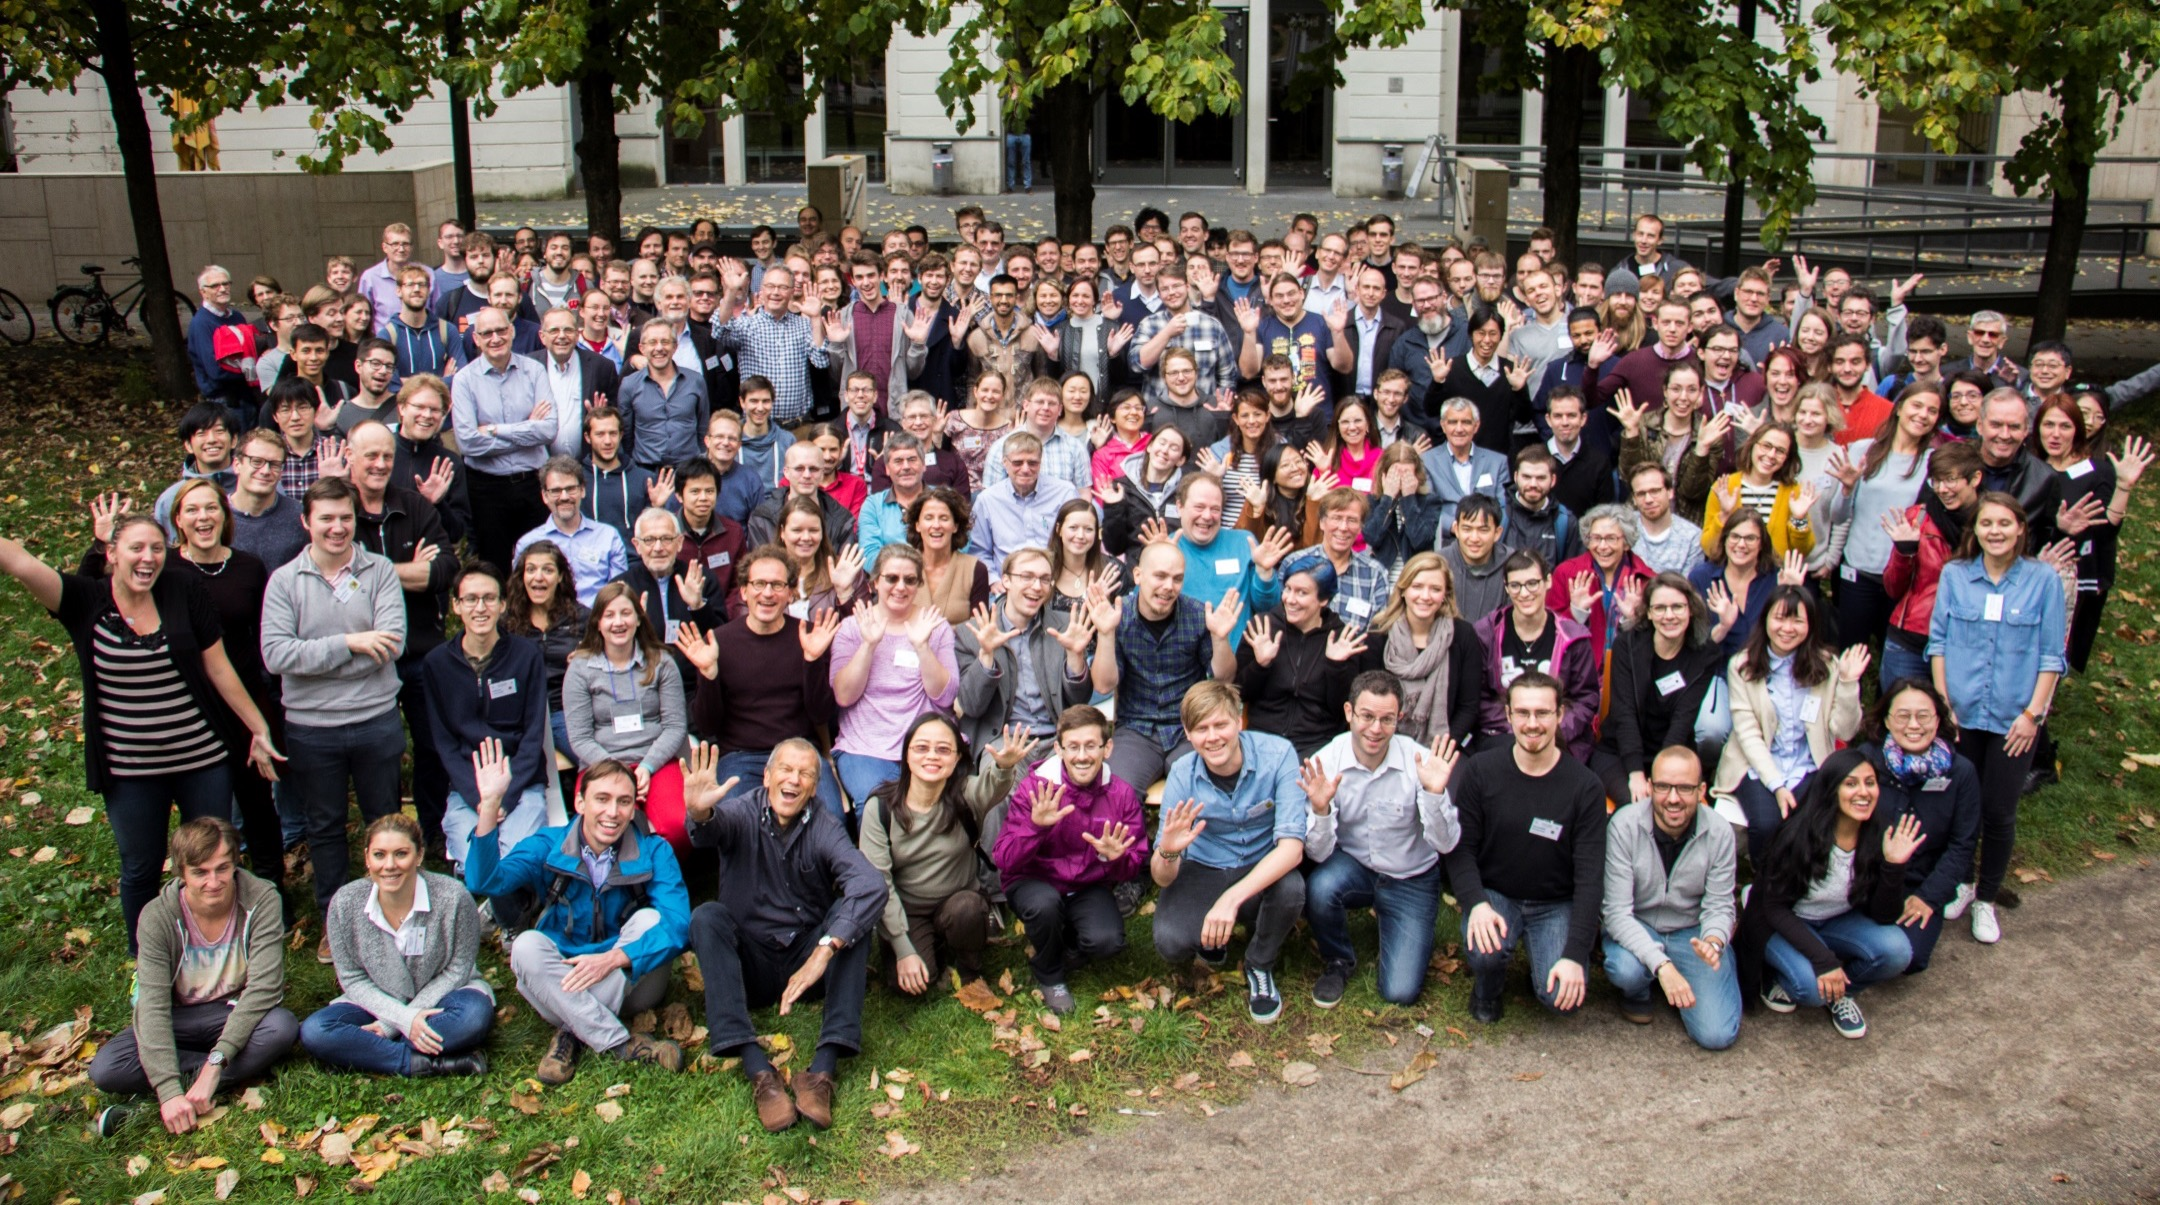
\includegraphics[width=0.94\linewidth]{halzen/icecube_colaboracion_foto.jpg}\\[1pt]
      {\scriptsize La colaboración IceCube}
    \column{0.42\textwidth}
      \small
      \begin{tcolorbox}[colback=itedaTeal, colframe=itedaTeal, arc=2pt,
        fontupper=\color{white}\small, before upper={\raggedright}]
        «Por sus contribuciones decisivas al Observatorio de Neutrinos IceCube
        y al descubrimiento de neutrinos de alta energía de origen
        astrofísico.»\\[2pt]
        {\footnotesize Real Academia Sueca de Ciencias, 6 de octubre de 2026}
      \end{tcolorbox}
      \vspace{2pt}
      {\footnotesize Impulsó el \textbf{hielo del Polo Sur} como detector
      (AMANDA, IceCube). 2013: neutrinos \textbf{astrofísicos}.}
  \end{columns}
  \credito{Foto: Colaboración IceCube, vía F.~Halzen (2024). Cita traducida de NobelPrize.org}
\end{frame}

% ---------------------------------------------------------------- 46
\begin{frame}[plain]
  \fondo[0.0]{halzen/halzen_p016_sintexto.jpg}
  \begin{tikzpicture}[remember picture, overlay]
    \node[anchor=north west, text=white, font=\Large\bfseries]
      at ([xshift=0.6cm, yshift=-0.35cm]current page.north west)
      {Otra vez Cherenkov, ahora en el hielo};
    \tikzset{rot/.style={font=\small, align=left, text=white}}
    \node[rot, anchor=west] at ([xshift=12.4cm, yshift=1.05cm]current page.south west)
      {$\nu_\mu + N \to \mu + X$\\{\footnotesize el $\nu$ no deja luz}};
    \node[rot, anchor=east] at ([xshift=8.7cm, yshift=2.6cm]current page.south west)
      {\textbf{muón}: km de traza\\emitiendo luz};
    \node[rot, anchor=east] at ([xshift=3.4cm, yshift=5.3cm]current page.south west)
      {módulos\\ópticos};
    \node[anchor=north east, fill=white, rounded corners=3pt, inner sep=2pt]
      at ([xshift=-0.4cm, yshift=-0.5cm]current page.north east)
      {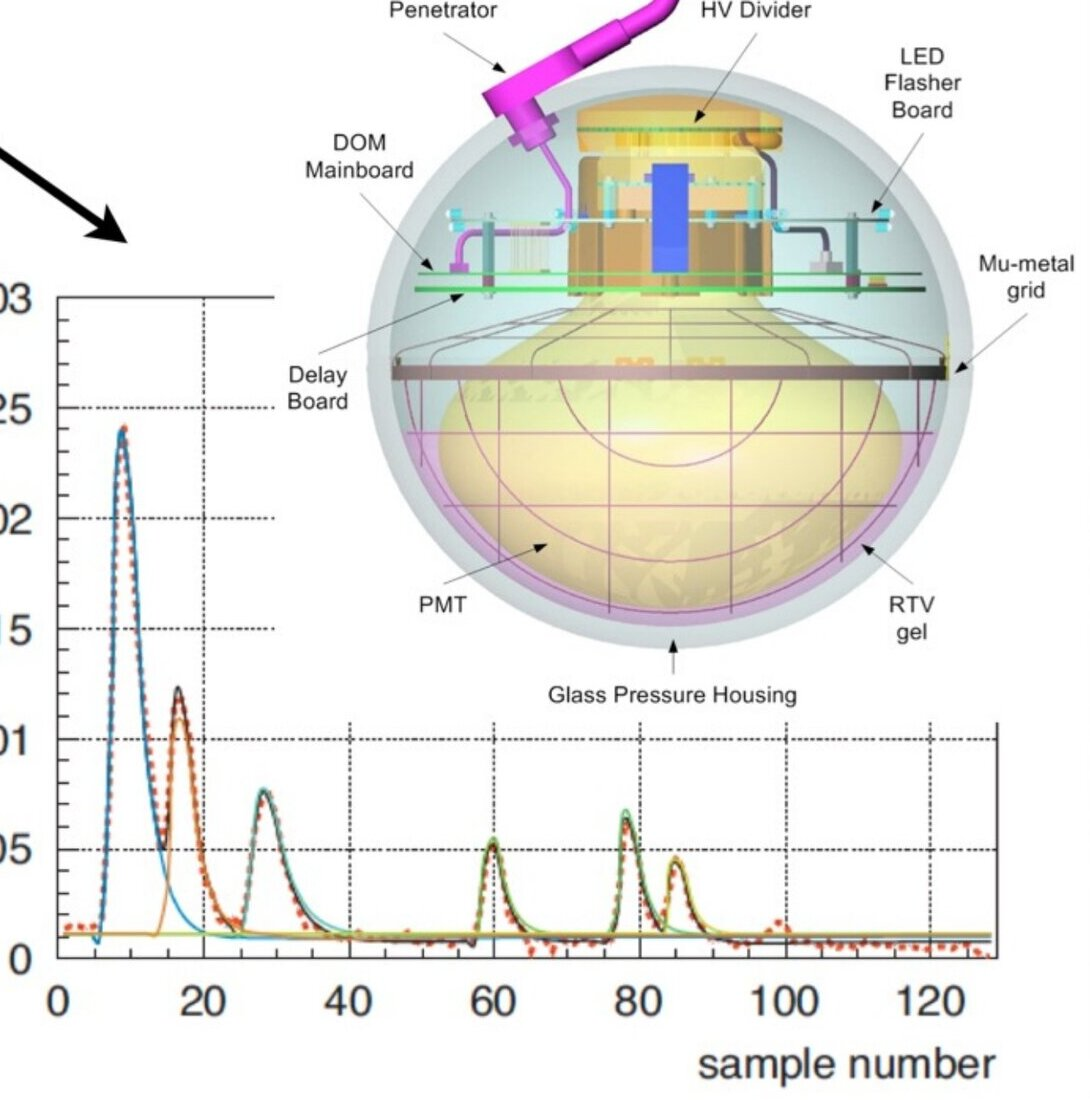
\includegraphics[height=3.4cm]{halzen/dom_formas_onda.jpg}};
    \node[anchor=north east, text width=4.9cm, align=left, text=white, font=\footnotesize]
      at ([xshift=-0.4cm, yshift=-4.1cm]current page.north east) {%
      Cada módulo \textbf{digitaliza} la forma de onda y le pone tiempo con
      precisión de nanosegundos. Con $\theta_C\approx41^\circ$ en el hielo, el
      \textbf{patrón de tiempos} da la dirección del muón.};
  \end{tikzpicture}
  \creditoblanco{Composición e inserto: F.~Halzen, Erice 2024}
\end{frame}

% ---------------------------------------------------------------- 47
\begin{frame}{Trazas y cascadas}
  \begin{columns}[T,onlytextwidth]
    \column{0.50\textwidth}
      \centering
      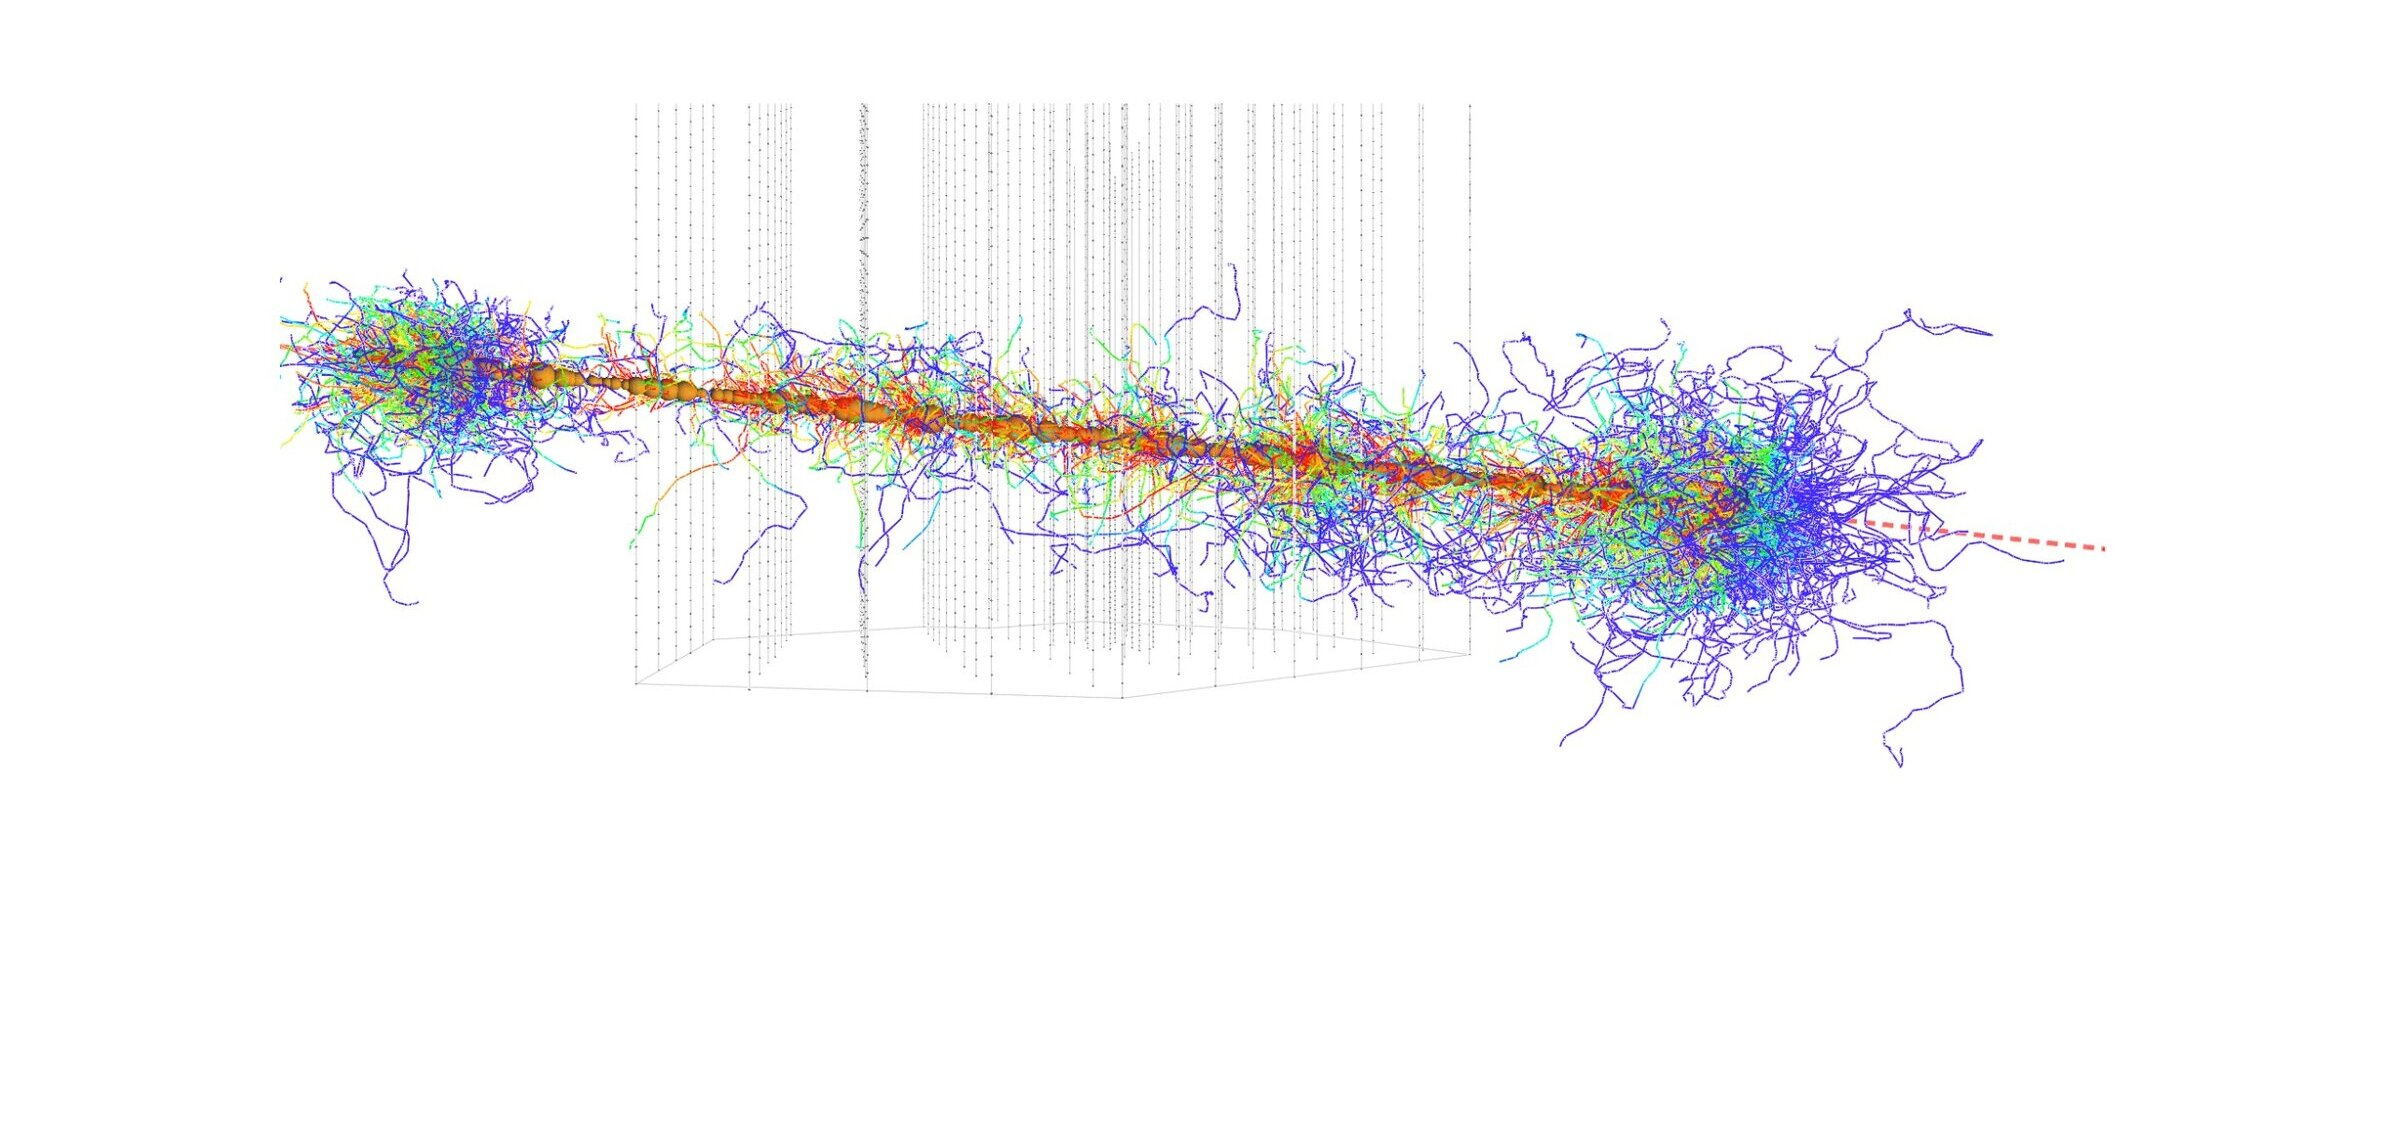
\includegraphics[height=3.0cm]{halzen/icecube_traza_r.jpg}\\[3pt]
      {\small\bfseries Traza}: $\nu_\mu$ por corriente cargada\\[2pt]
      {\footnotesize Muón de kilómetros: \textbf{dirección} con
      resolución $\lesssim1^\circ$ (hasta $\sim$0,3$^\circ$), pero sólo
      parte de la energía queda adentro.}
    \column{0.47\textwidth}
      \centering
      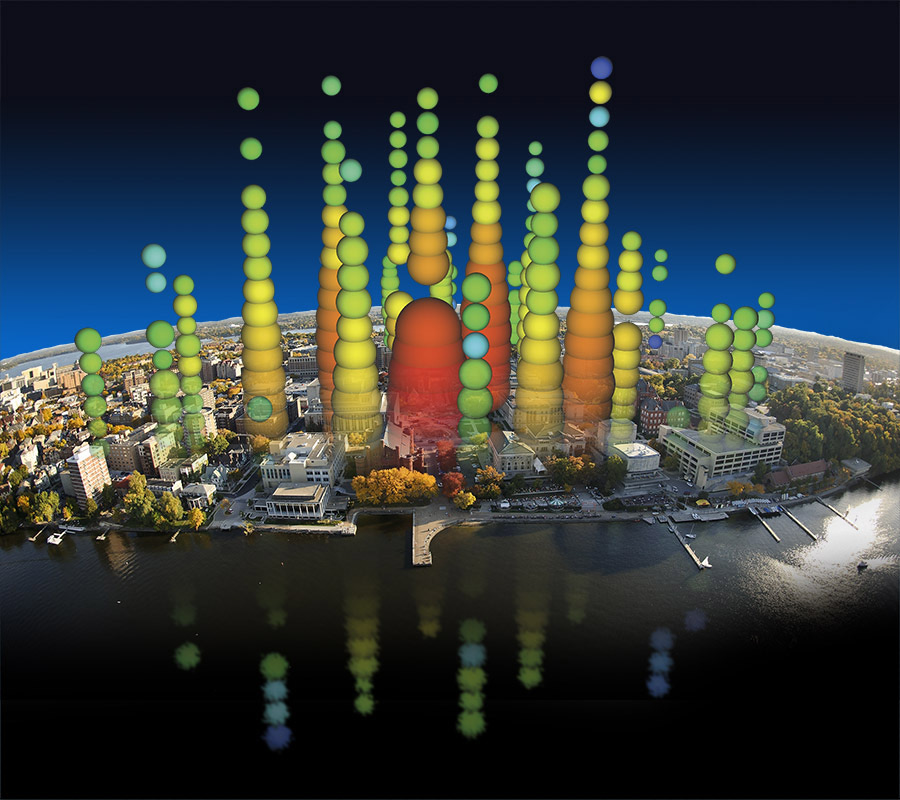
\includegraphics[height=3.0cm]{halzen/icecube_cascada_escala.jpg}\\[3pt]
      {\small\bfseries Cascada}: $\nu_e$, $\nu_\tau$ y corriente neutra\\[2pt]
      {\footnotesize Unos 10\,m de lluvia en el hielo: casi esférica vista de
      lejos. \textbf{Energía} a $\sim$10\%, dirección de $\sim$10$^\circ$.}
  \end{columns}
  \vspace{4pt}
  \begin{clave}
    Las trazas \textbf{apuntan}; las cascadas \textbf{miden energía}.
  \end{clave}
  \credito{Eventos de IceCube, vía F.~Halzen (2024). Derecha: cascada de PeV junto a edificios, para dar escala}
\end{frame}

% ---------------------------------------------------------------- 48
\begin{frame}{Una década de descubrimientos}
  \begin{columns}[T,onlytextwidth]
    \column{0.24\textwidth}
      \centering
      {\footnotesize\bfseries 2013 · flujo difuso}\\[2pt]
      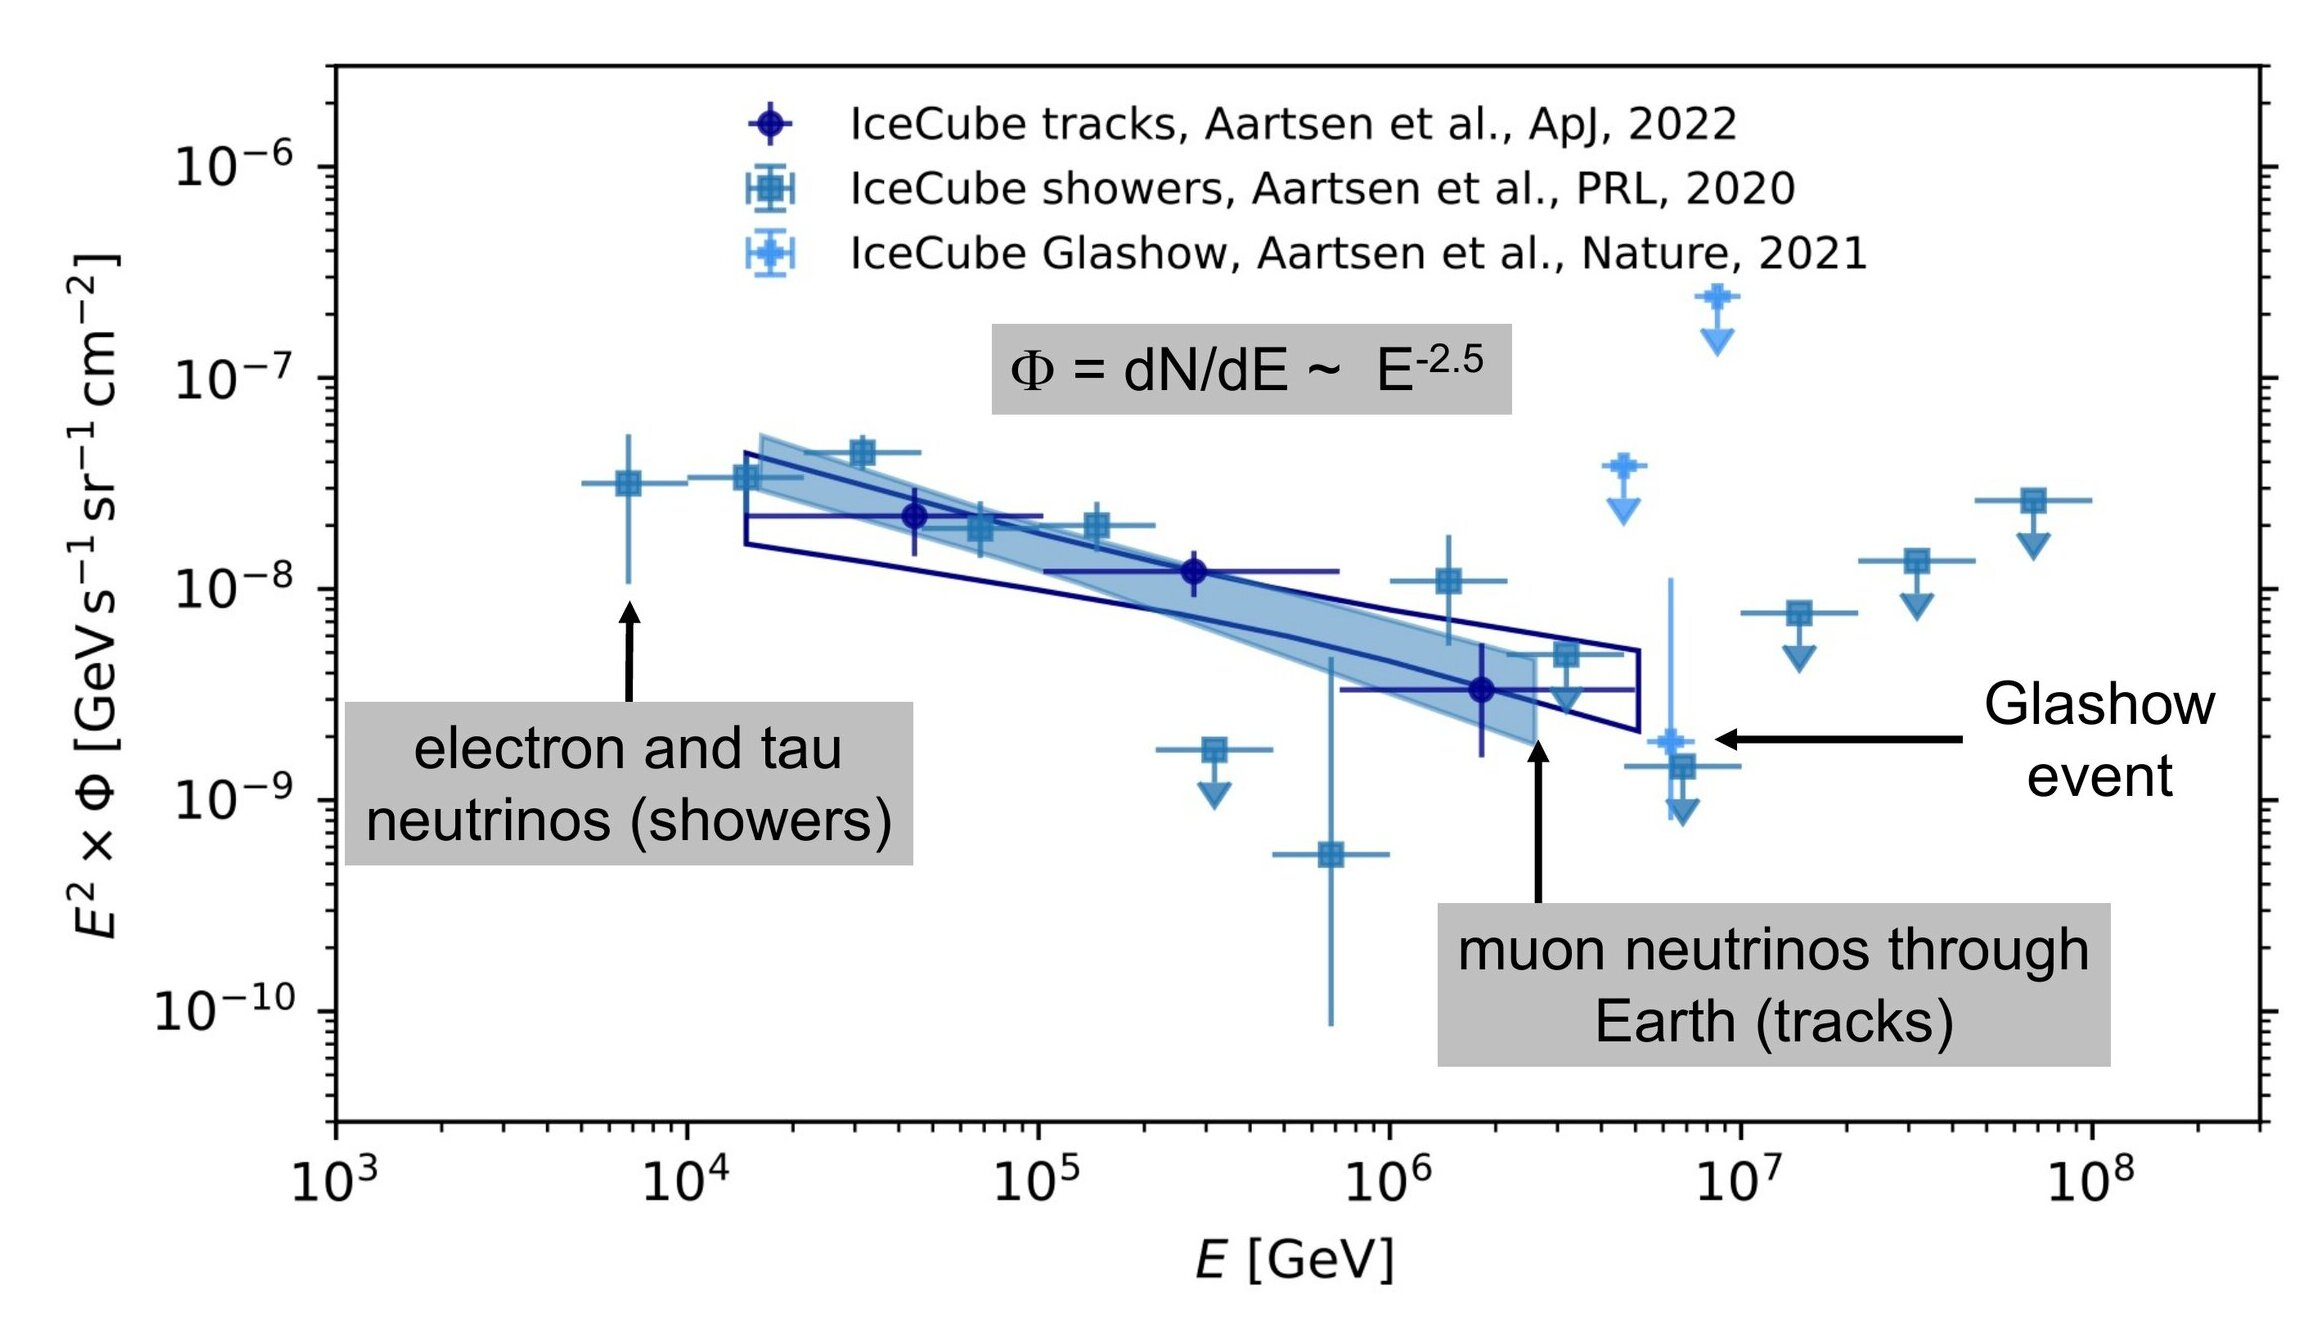
\includegraphics[width=\linewidth]{halzen/flujo_difuso.jpg}\\[2pt]
      {\scriptsize Neutrinos de TeV--PeV de origen \textbf{astrofísico}, espectro
      $\sim E^{-2,5}$.}
    \column{0.24\textwidth}
      \centering
      {\footnotesize\bfseries 2017 · TXS 0506+056}\\[2pt]
      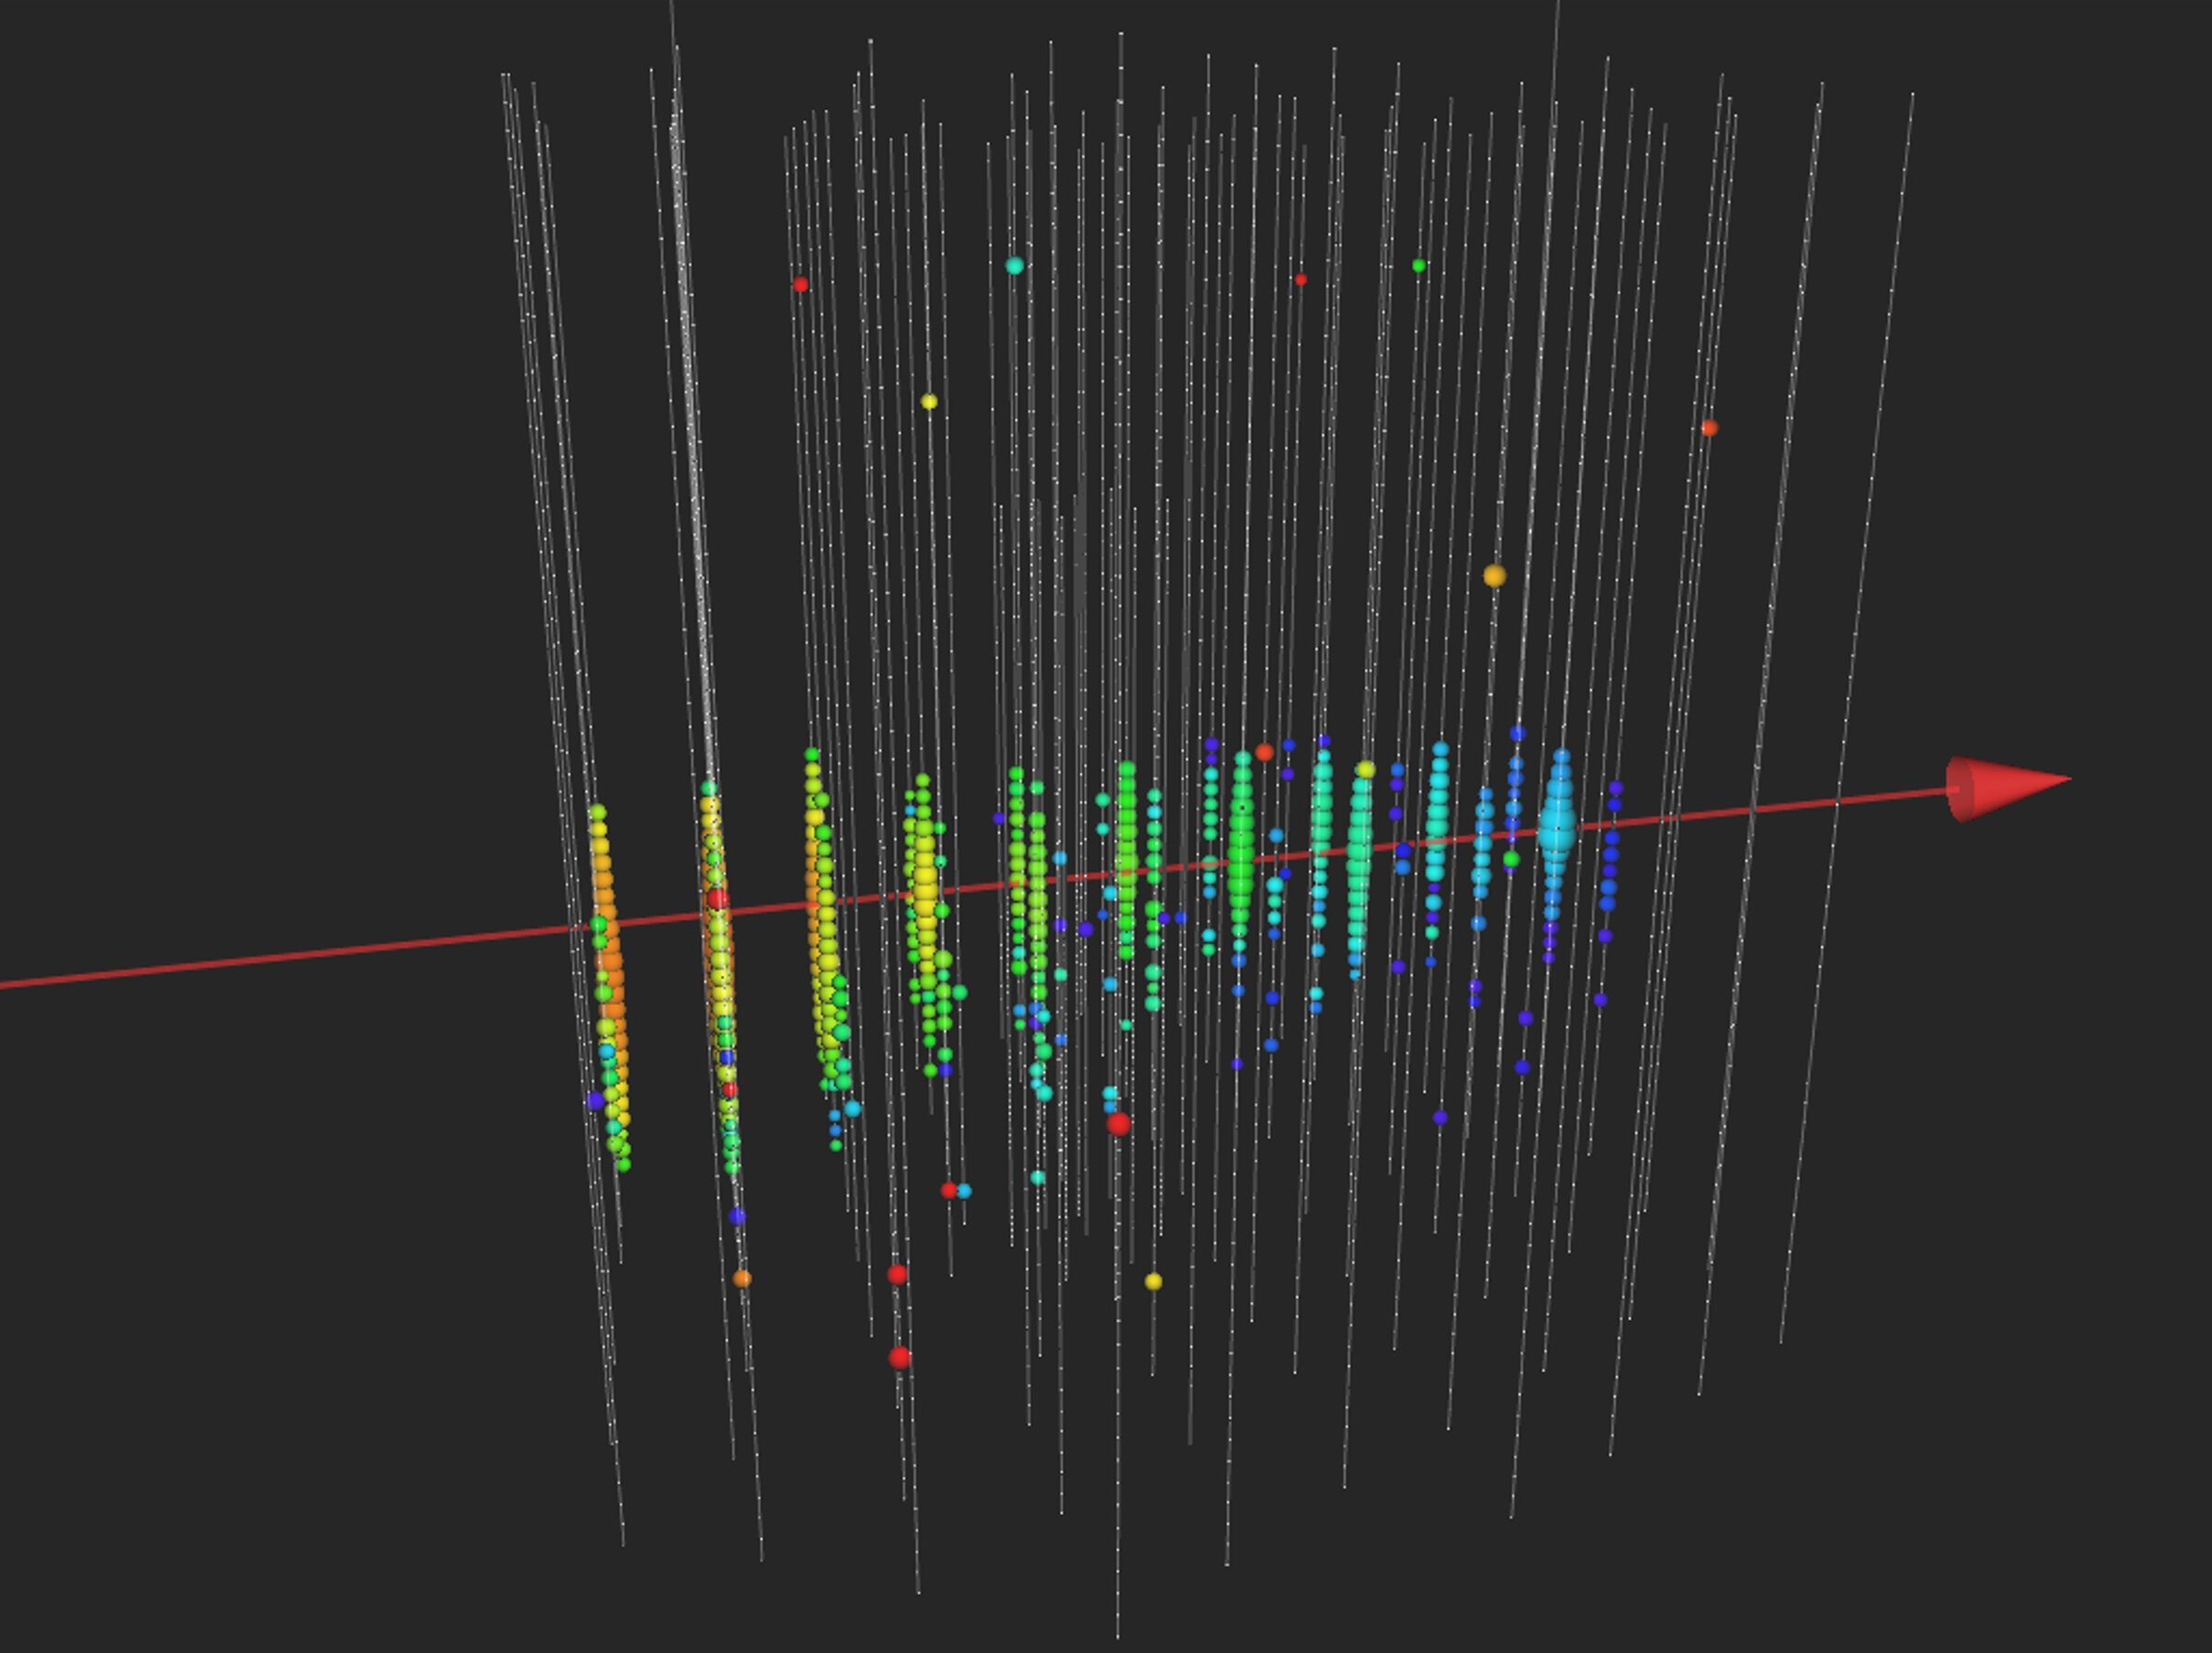
\includegraphics[width=\linewidth]{halzen/icecube_ic170922a.jpg}\\[2pt]
      {\scriptsize Un neutrino de $\sim$290\,TeV coincide con un blazar en
      \textbf{erupción gamma}.}
    \column{0.24\textwidth}
      \centering
      {\footnotesize\bfseries 2022 · NGC 1068}\\[2pt]
      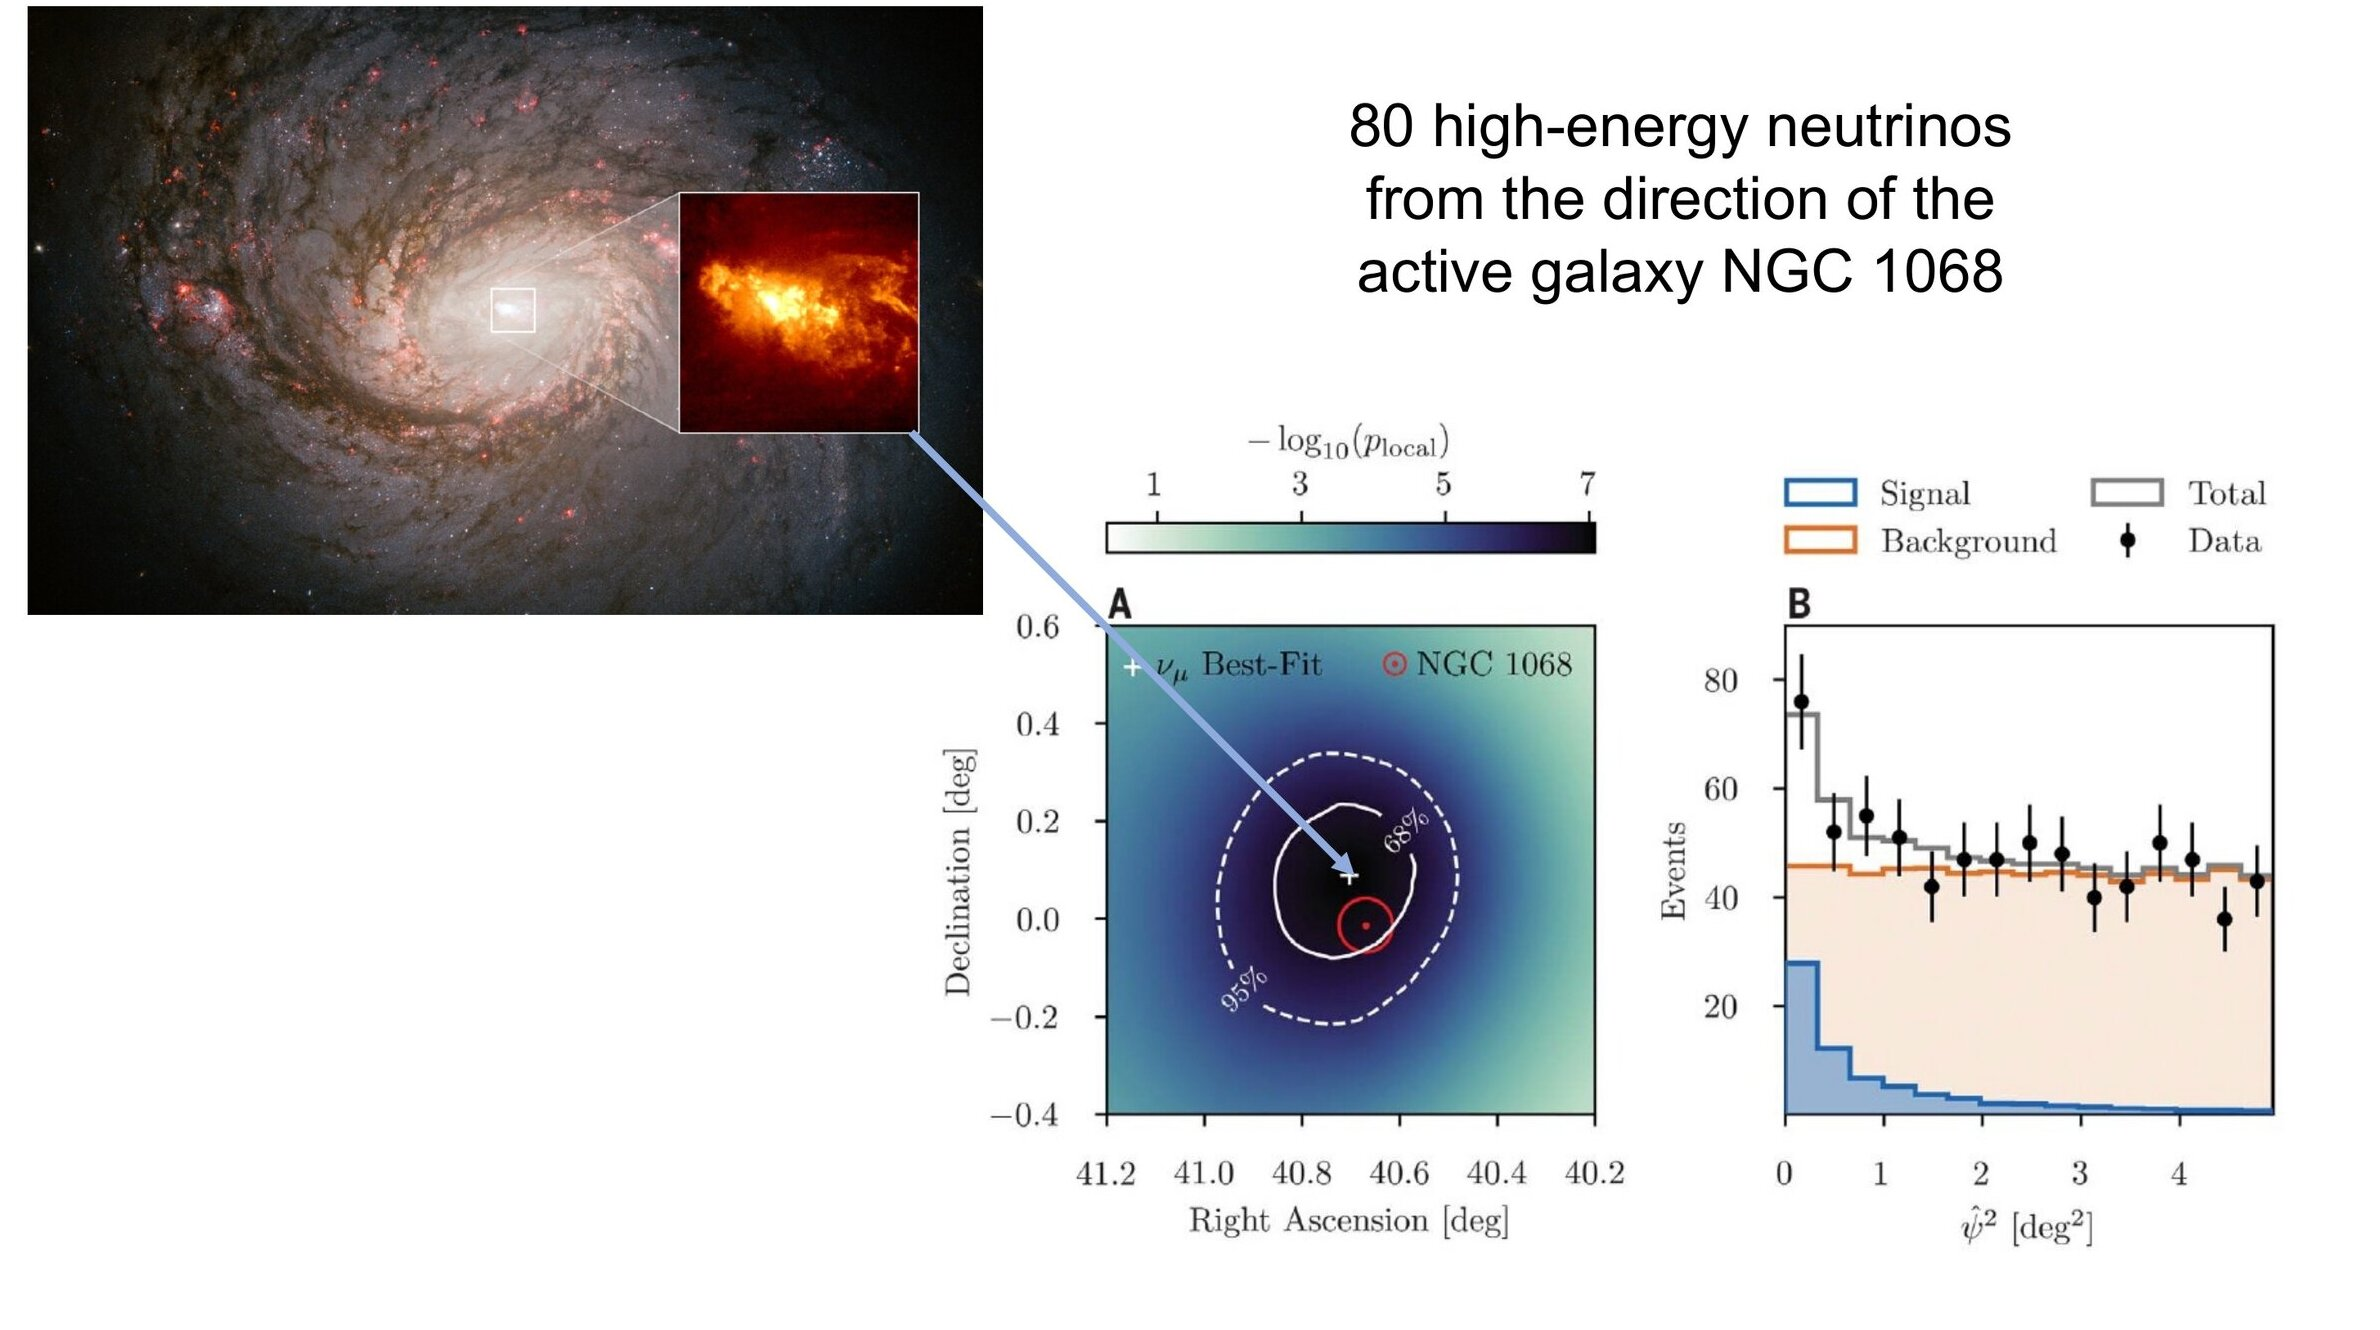
\includegraphics[width=\linewidth]{halzen/ngc1068.jpg}\\[2pt]
      {\scriptsize $\sim$80 neutrinos de una galaxia activa cercana, a
      4,2$\sigma$, \textbf{sin} gammas de TeV: núcleo opaco.}
    \column{0.24\textwidth}
      \centering
      {\footnotesize\bfseries 2023 · nuestra galaxia}\\[2pt]
      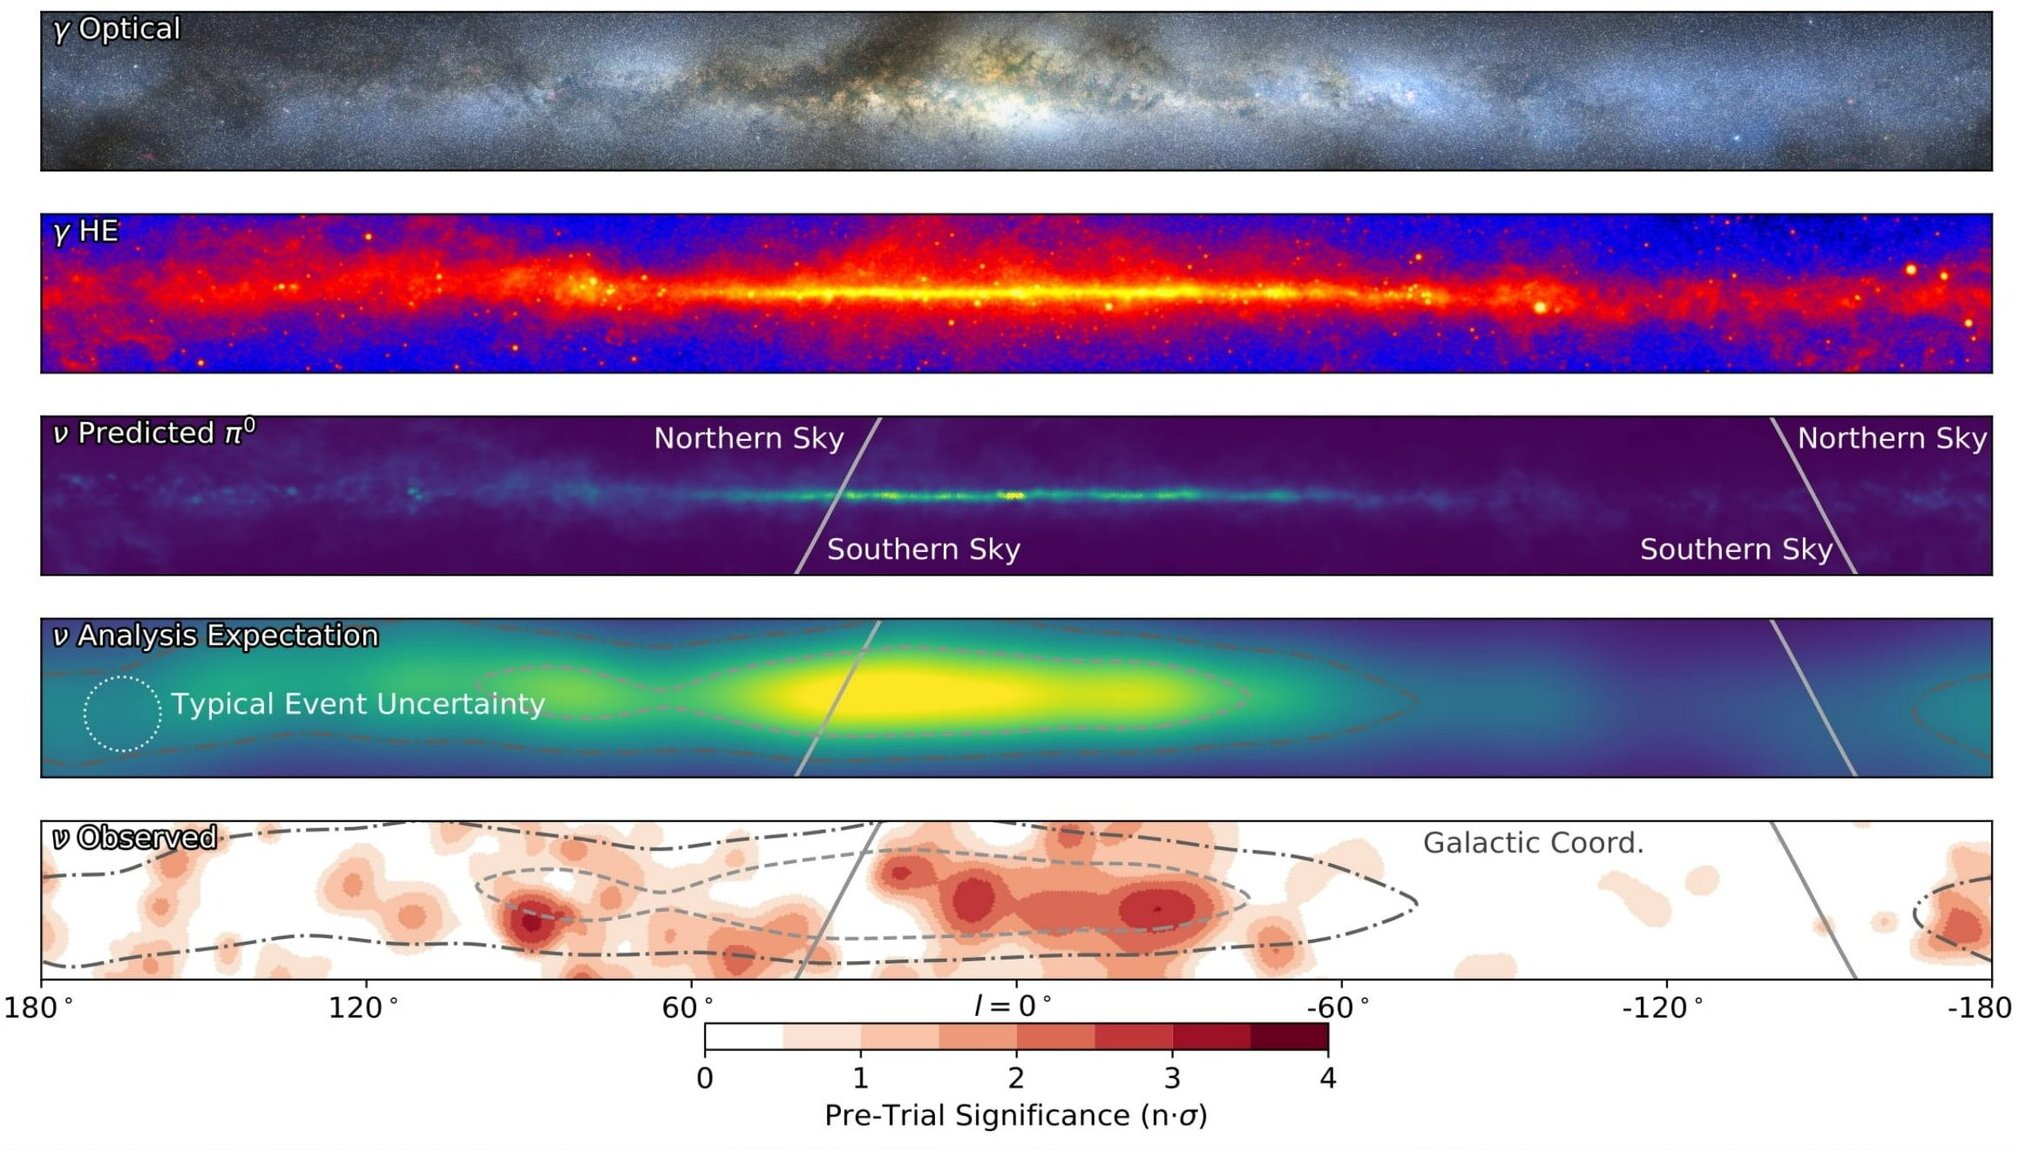
\includegraphics[width=\linewidth]{halzen/plano_galactico_fermi_icecube.jpg}\\[2pt]
      {\scriptsize El plano galáctico en neutrinos (4,5$\sigma$), como lo predicen
      los rayos cósmicos sobre el gas.}
  \end{columns}
  \vspace{6pt}
  \begin{clave}
    La fuente de neutrinos más clara no es la más brillante en gammas: los
    neutrinos ven \textbf{adentro} de los aceleradores.
  \end{clave}
  \credito{Figuras: Colaboración IceCube (Science 2013, 2018, 2022, 2023), vía F.~Halzen (2024)}
\end{frame}

% ---------------------------------------------------------------- 48b
\begin{frame}{NGC 1068: neutrinos desde el corazón de una galaxia activa}
  \begin{columns}[c,onlytextwidth]
    \column{0.55\textwidth}
      \centering
      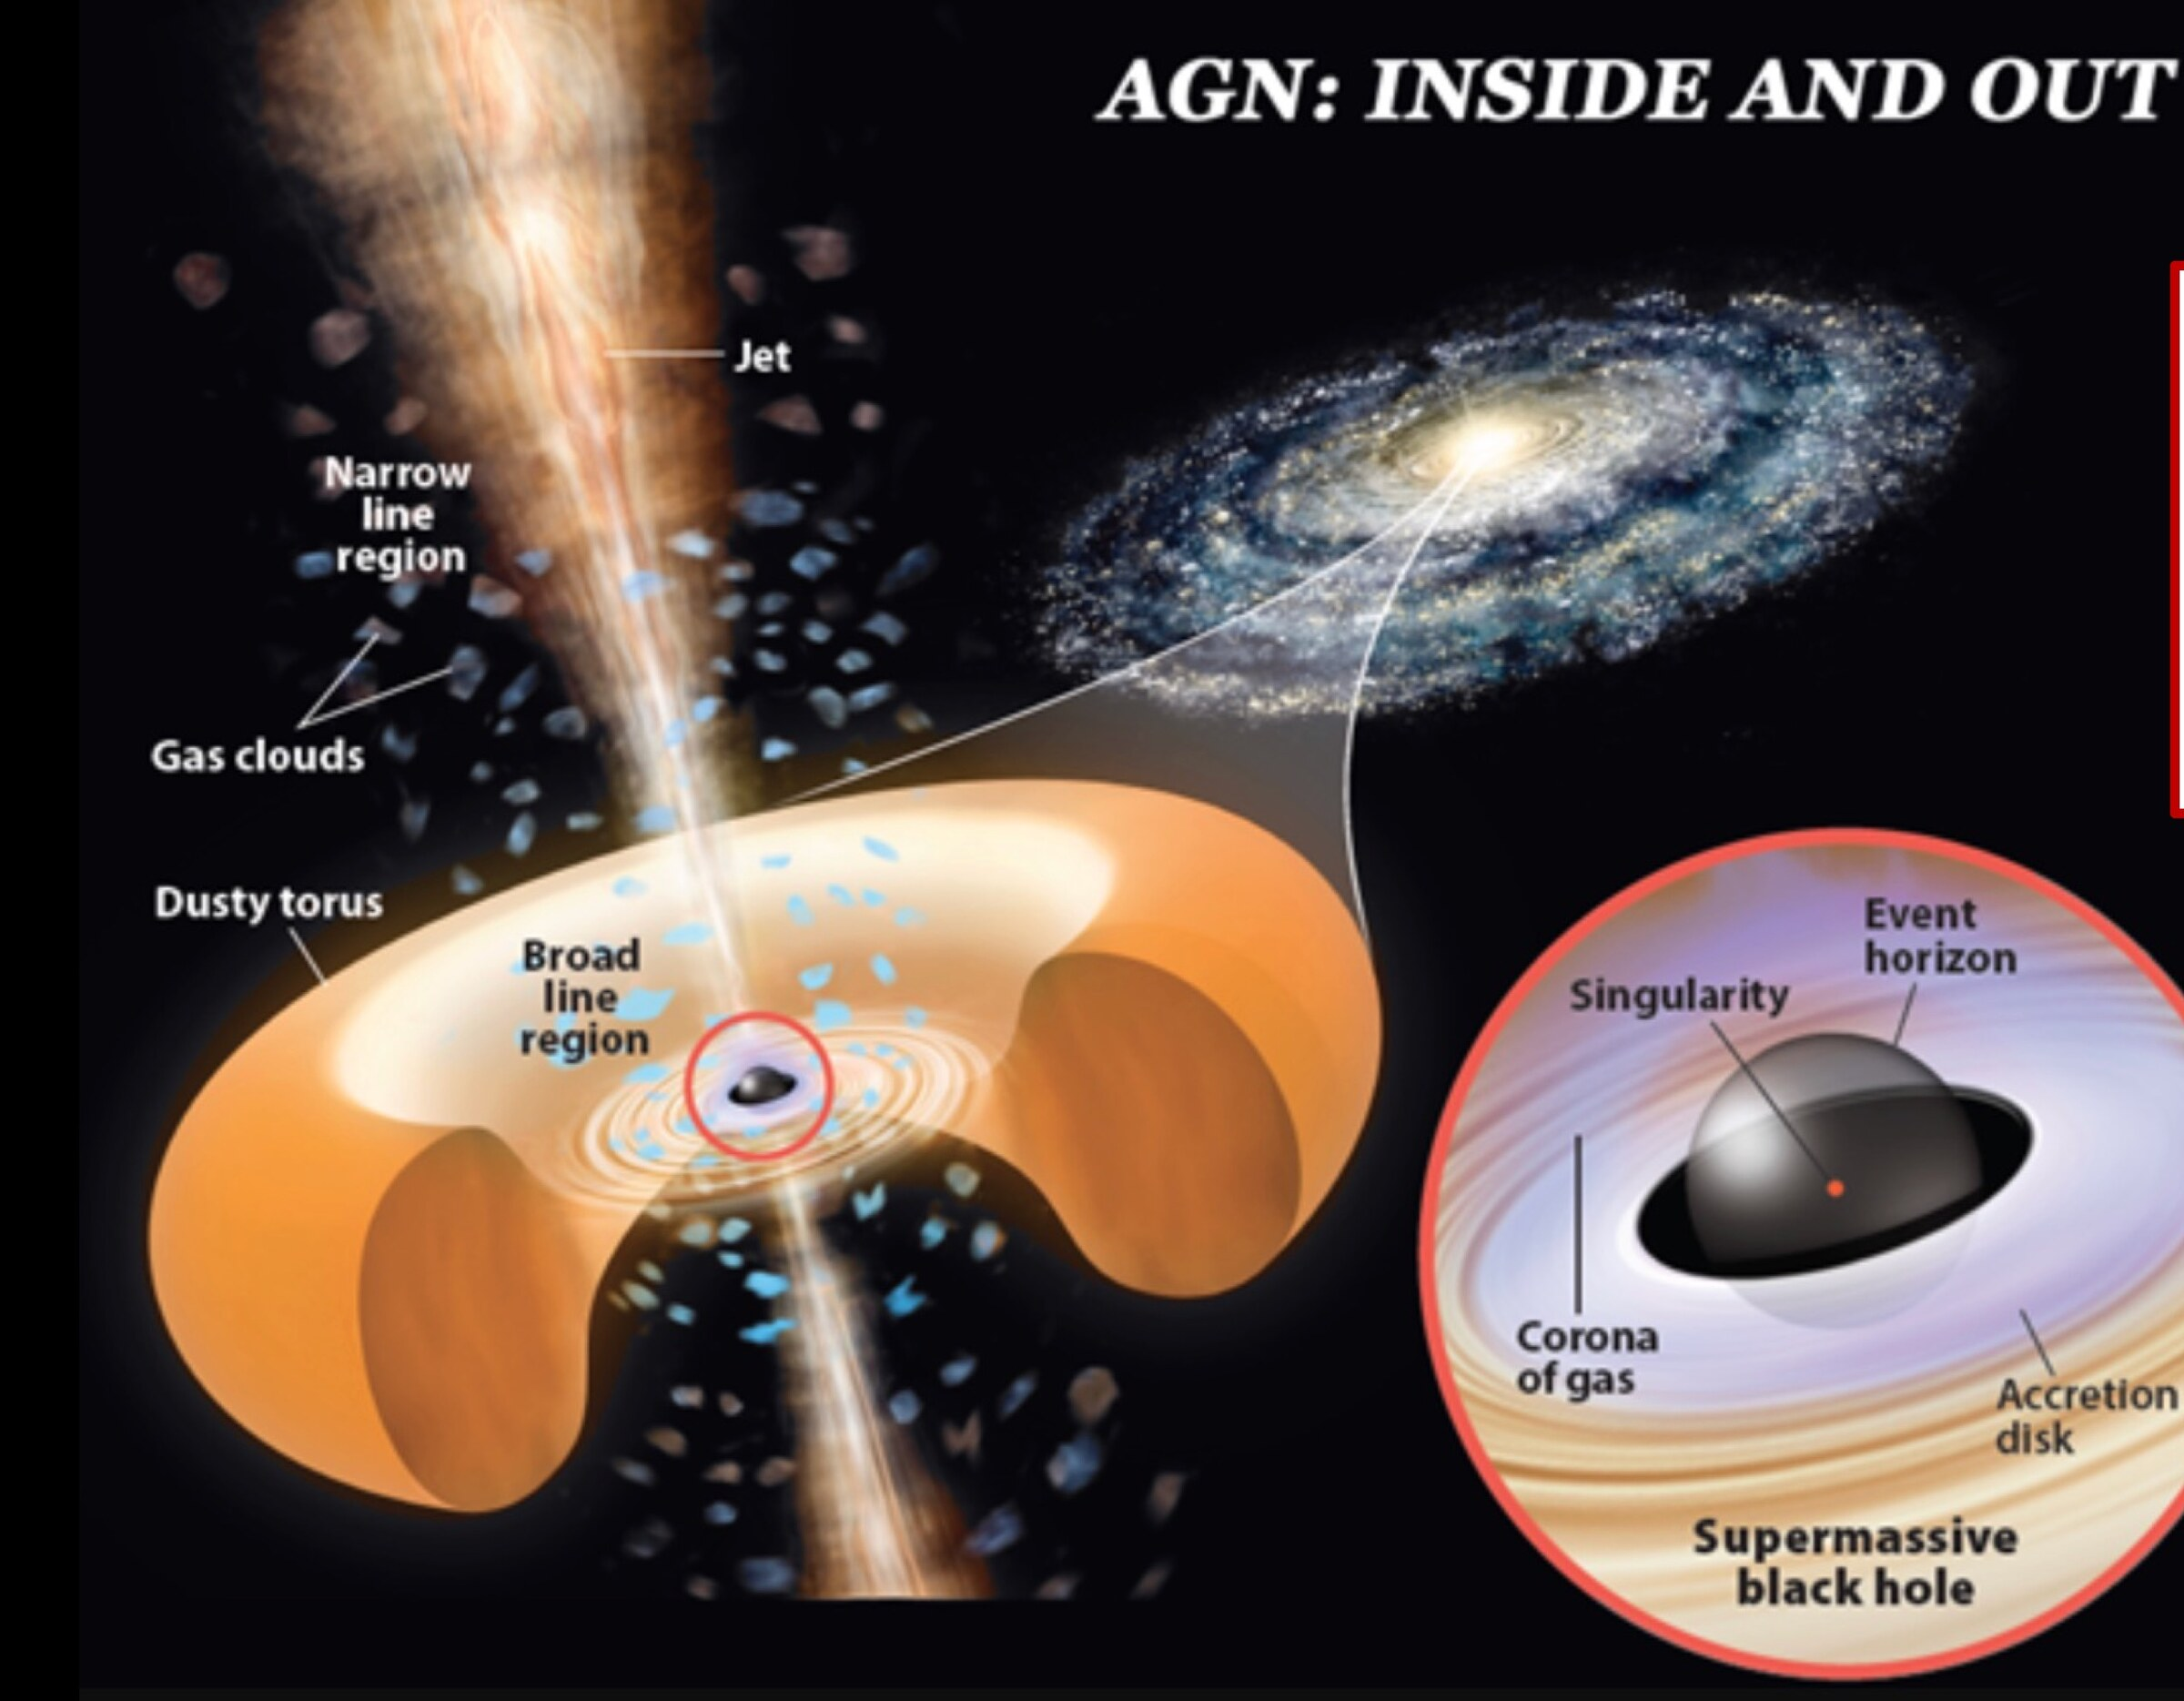
\includegraphics[width=\linewidth]{halzen/agn_inside_out.jpg}
    \column{0.42\textwidth}
      \footnotesize
      Un \textbf{núcleo galáctico activo} (AGN): un agujero negro gigante que
      traga gas de un disco, rodeado por una \textbf{corona} caliente que
      brilla en rayos X.
      \vspace{2pt}
      \begin{itemize}\footnotesize
        \item IceCube vio $\sim$80 neutrinos de 1,5--15\,TeV desde NGC 1068
          (a $\sim$14\,Mpc), con 4,2$\sigma$.
        \item Pero \textbf{no llegan los gammas} que deberían acompañarlos.
      \end{itemize}
      \begin{clave}[fontupper=\footnotesize]
        Los gammas chocan con los rayos X de la corona y quedan atrapados; los
        neutrinos escapan. Se producen \textbf{muy cerca del agujero negro},
        donde la luz no sale.
      \end{clave}
  \end{columns}
  \creditoizq{Ilustración: «AGN: inside and out», vía F.~Halzen (2024). IceCube, Science 378 (2022) 538}
\end{frame}

% ---------------------------------------------------------------- 48c
\begin{frame}{La Vía Láctea vista con neutrinos}
  \begin{columns}[c,onlytextwidth]
    \column{0.55\textwidth}
      \centering
      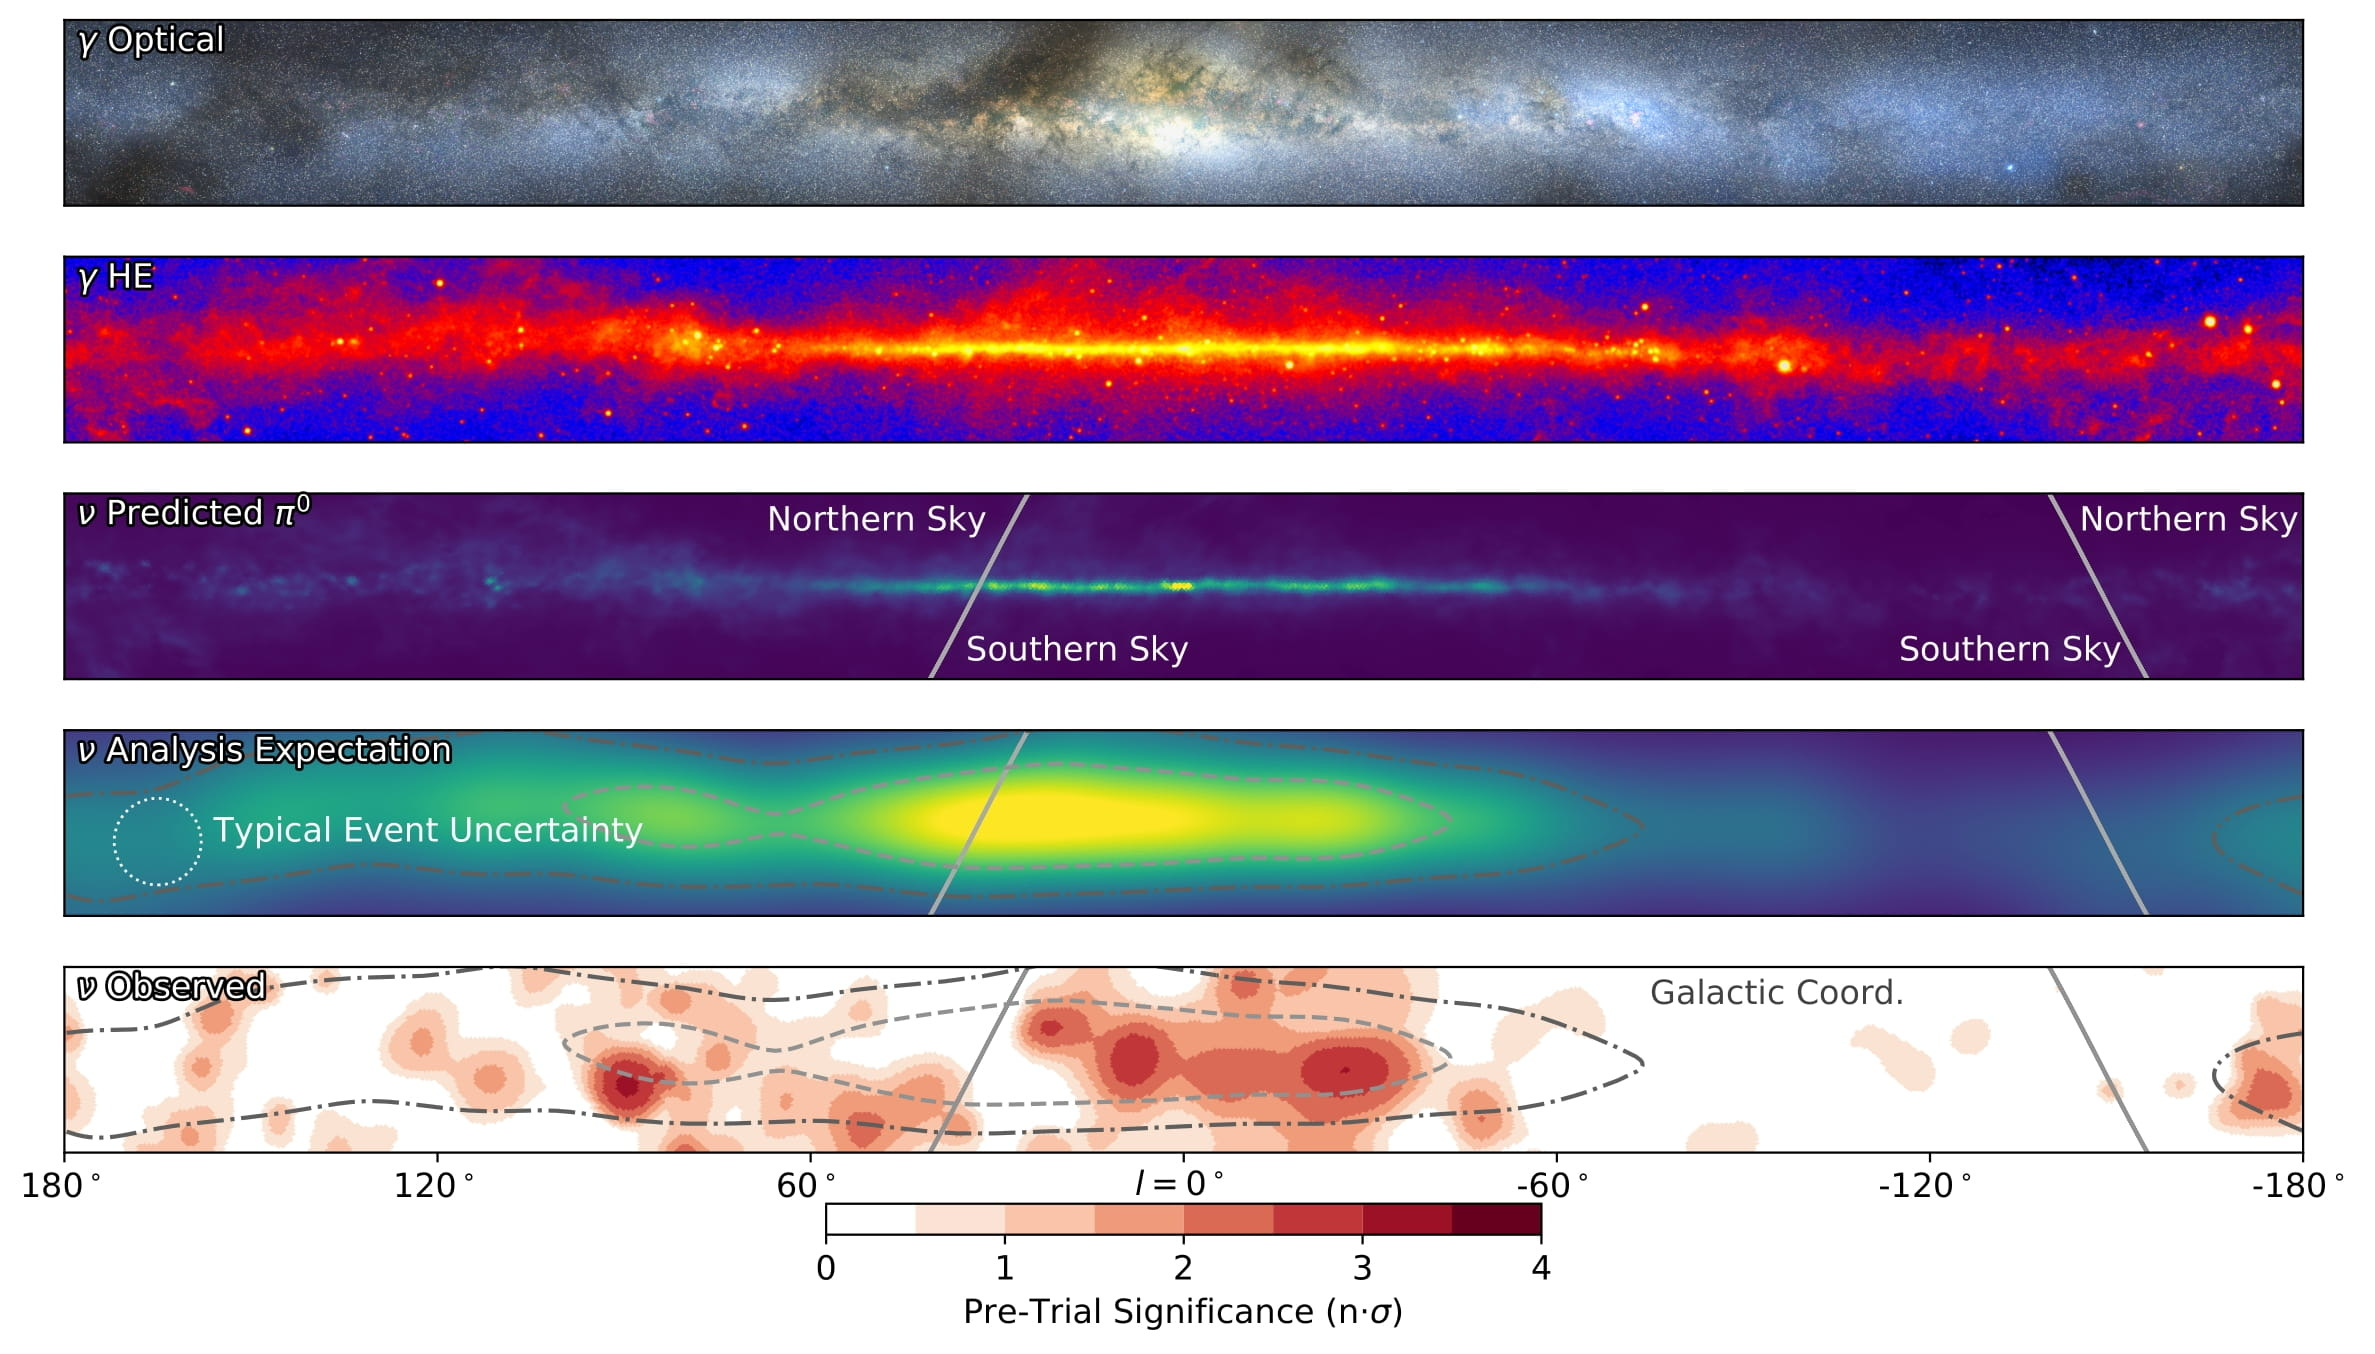
\includegraphics[width=\linewidth]{halzen/plano_galactico_paneles.jpg}
    \column{0.42\textwidth}
      \footnotesize
      De arriba a abajo: el plano de la galaxia en \textbf{luz visible}, en
      \textbf{rayos gamma} (Fermi), la \textbf{predicción} de neutrinos y lo
      que \textbf{observó} IceCube.
      \vspace{2pt}
      \begin{itemize}\footnotesize
        \item Los rayos cósmicos de la galaxia chocan con el gas interestelar:
          producen piones, que dan gammas \emph{y} neutrinos.
        \item IceCube encontró esa emisión a lo largo del plano (no sólo del
          centro), con 4,5$\sigma$ (2023).
      \end{itemize}
      \begin{clave}[fontupper=\footnotesize]
        La primera imagen de nuestra galaxia en neutrinos, como predicen los
        rayos cósmicos.
      \end{clave}
  \end{columns}
  \creditoizq{IceCube, Science 380 (2023) 1338, vía F.~Halzen (2024)}
\end{frame}

% ---------------------------------------------------------------- 49
\begin{frame}{Auger e IceCube: dos instrumentos, dos problemas}
  \begin{tikzpicture}[x=1cm,y=1cm]
    \tikzset{
      cab/.style={font=\small\bfseries, text=white, minimum width=5.6cm,
        minimum height=0.6cm, rounded corners=2pt},
      fila/.style={font=\footnotesize, text width=5.2cm, align=left, anchor=north west},
      lab/.style={font=\scriptsize\bfseries, text=itedaGray, anchor=north east, align=right}}
    \node[cab, fill=itedaOrange] at (5.2,0) {Pierre Auger};
    \node[cab, fill=cmbAzul] at (11.1,0) {IceCube};
    \foreach \y/\l/\a/\b in {
        -0.5/{Geometría}/{Superficie de 3000\,km$^2$}/{Volumen de 1\,km$^3$},
        -1.15/{Qué detecta}/{Lluvias de rayos cósmicos}/{Secundarios de interacciones de $\nu$},
        -1.8/{Cherenkov}/{Agua: \textbf{muestrea} la lluvia}/{Hielo: \textbf{blanco y calorímetro}},
        -2.45/{Energías}/{$\gtrsim10^{17}$\,eV}/{$10^{10}$ a $10^{16}$\,eV (10\,GeV a 10\,PeV)},
        -3.1/{Fortaleza}/{Exposición a lo más raro}/{Direcciones y sabores de $\nu$}}{
      \node[lab] at (2.35,\y) {\l};
      \node[fila] at (2.55,\y) {\a};
      \node[fila] at (8.45,\y) {\b};
      \draw[itedaGray!30] (0.4,\y+0.08) -- (13.9,\y+0.08);}
  \end{tikzpicture}\\[2pt]
  {\footnotesize\color{itedaGray} Auger también busca $\nu$ muy inclinados;
  IceCube también registra muones atmosféricos y lluvias (IceTop).}\\[2pt]
  {\scriptsize\color{itedaTealDark}\textbf{Prefijos:} G (giga) $=10^9$ \quad T (tera) $=10^{12}$
  \quad P (peta) $=10^{15}$ \quad E (exa) $=10^{18}$}\\[3pt]
  \begin{clave}
    La aceptación de cada uno sale de su \textbf{blanco} (atmósfera o hielo)
    y de su \textbf{umbral}: a 1\,PeV, un neutrino interactúa en 1\,km de hielo
    con probabilidad $\sim5\times10^{-5}$.
  \end{clave}
\end{frame}

% ---------------------------------------------------------------- 50
\begin{frame}{Astronomía multimensajero}
  \begin{columns}[c,onlytextwidth]
    \column{0.47\textwidth}
      \centering
      \begin{tikzpicture}[x=1cm,y=1cm]
        \shade[ball color=black!80] (0,0) circle (0.35);
        \fill[itedaOrange!60] (-0.1,0.3) -- (0.1,0.3) -- (0.35,2.0) -- (-0.35,2.0) -- cycle;
        \node[font=\scriptsize, text=itedaGray] at (0,-0.6) {fuente};
        \draw[very thick, itedaOrange, -{Stealth}] (0.4,0.1) .. controls (1.5,1.6) and (2.2,-1.3) .. (4.0,0.9);
        \node[font=\scriptsize, text=itedaOrange, anchor=west, align=left] at (4.05,0.9) {rayos\\cósmicos};
        \draw[very thick, cmbAzul, -{Stealth}] (0.4,-0.2) -- (2.8,-0.45);
        \node[font=\scriptsize, text=cmbAzul] at (3.0,-0.47) {$\times$};
        \node[font=\scriptsize, text=cmbAzul, anchor=west] at (3.2,-0.47) {fotones};
        \draw[very thick, violetaNu, -{Stealth}] (0.4,-0.45) -- (4.0,-1.2);
        \node[font=\scriptsize, text=violetaNu, anchor=west] at (4.05,-1.2) {neutrinos};
        \draw[very thick, verdeRadio, -{Stealth}, decorate, decoration={snake, amplitude=1mm,
          segment length=4mm, post length=2mm}] (0.4,-0.7) -- (4.0,-1.95);
        \node[font=\scriptsize, text=verdeRadio, anchor=west, align=left] at (4.05,-1.95) {ondas\\gravitac.};
      \end{tikzpicture}\\[4pt]
      {\footnotesize Cada mensajero interactúa distinto \textbf{en la fuente} y
      \textbf{en el camino}: juntos reconstruyen el acelerador.}
    \column{0.50\textwidth}
      \small
      \textbf{GW170817}: dos estrellas de neutrones a $\sim$40\,Mpc.
      \vspace{2pt}

      \begin{tikzpicture}[x=1cm,y=1cm]
        \draw[itedaGray, thick] (0,0) -- (0,-3.6);
        \foreach \y/\t/\d in {0/{$t_0$}/{ondas gravitacionales (LIGO--Virgo)},
          -0.9/{+1,7\,s}/{estallido de rayos gamma (Fermi, INTEGRAL)},
          -1.8/{+11\,h}/{kilonova óptica en NGC 4993},
          -2.7/{+9\,d}/{rayos X},
          -3.6/{+16\,d}/{radio}}{
          \fill[itedaOrange] (0,\y) circle (2.2pt);
          \node[font=\scriptsize\bfseries, anchor=east] at (-0.15,\y) {\t};
          \node[font=\scriptsize, anchor=west] at (0.15,\y) {\d};}
      \end{tikzpicture}\\[4pt]
      {\footnotesize IceCube, ANTARES y \textbf{Auger} buscaron neutrinos:
      ninguno, compatible con un chorro visto de costado.}
  \end{columns}
  \credito{LIGO--Virgo \textit{et al.}, ApJL 848 (2017) L12; ANTARES, IceCube y Auger, ApJL 850 (2017) L35}
\end{frame}
